\documentclass[10pt]{scrartcl}

\usepackage[utf8]{inputenc}
\usepackage{tabularx}
\usepackage[ngerman]{babel}
\usepackage[automark]{scrpage2}
\usepackage{amsmath,amssymb,amstext}
%\usepackage{mathtools}
\usepackage[]{color}
\usepackage[]{enumerate}
\usepackage{graphicx}
\usepackage{lastpage}
\usepackage[perpage,para,symbol*]{footmisc}
\usepackage{listings} 
\usepackage[pdfborder={0 0 0},colorlinks=false]{hyperref}
\usepackage[numbers,square]{natbib}
\usepackage{color}
\usepackage{colortbl}
\usepackage{listings}
\usepackage{a4wide}
\usepackage{xspace}
\usepackage{listings}
\usepackage{hyperref}
\usepackage{epstopdf}

\lstset{numbers=left, numberstyle=\tiny, numbersep=5pt, breaklines=true, showstringspaces=false} 

%changehere
\def\titletext{TH1 Praktikum 1 : Ausarbeitung}
\def\titletextshort{Praktikum 1}
\author{Carsten Noetzel, Armin Steudte}

\title{\titletext}

%changehere Datum der Übung
\date{23.03.2012}

\pagestyle{scrheadings}
%changehere
\ihead{TH1, Padberg}
\ifoot{Generiert am:\\ \today}

\cfoot{Carsten Noetzel, Armin Steudte}


\ohead[]{\titletextshort}
\ofoot[]{{\thepage} / \pageref{LastPage}}

\setlength{\parindent}{0.0in}
\setlength{\parskip}{0.1in}

\begin{document}
\maketitle

\setcounter{tocdepth}{3}
\tableofcontents
\listoffigures
%\lstlistoflistings

\section{Aufgabe 1 bis 4  - Alternating Bit Protokoll}
\subsection{Das Modell}
\begin{figure}[htbp]
	\centering	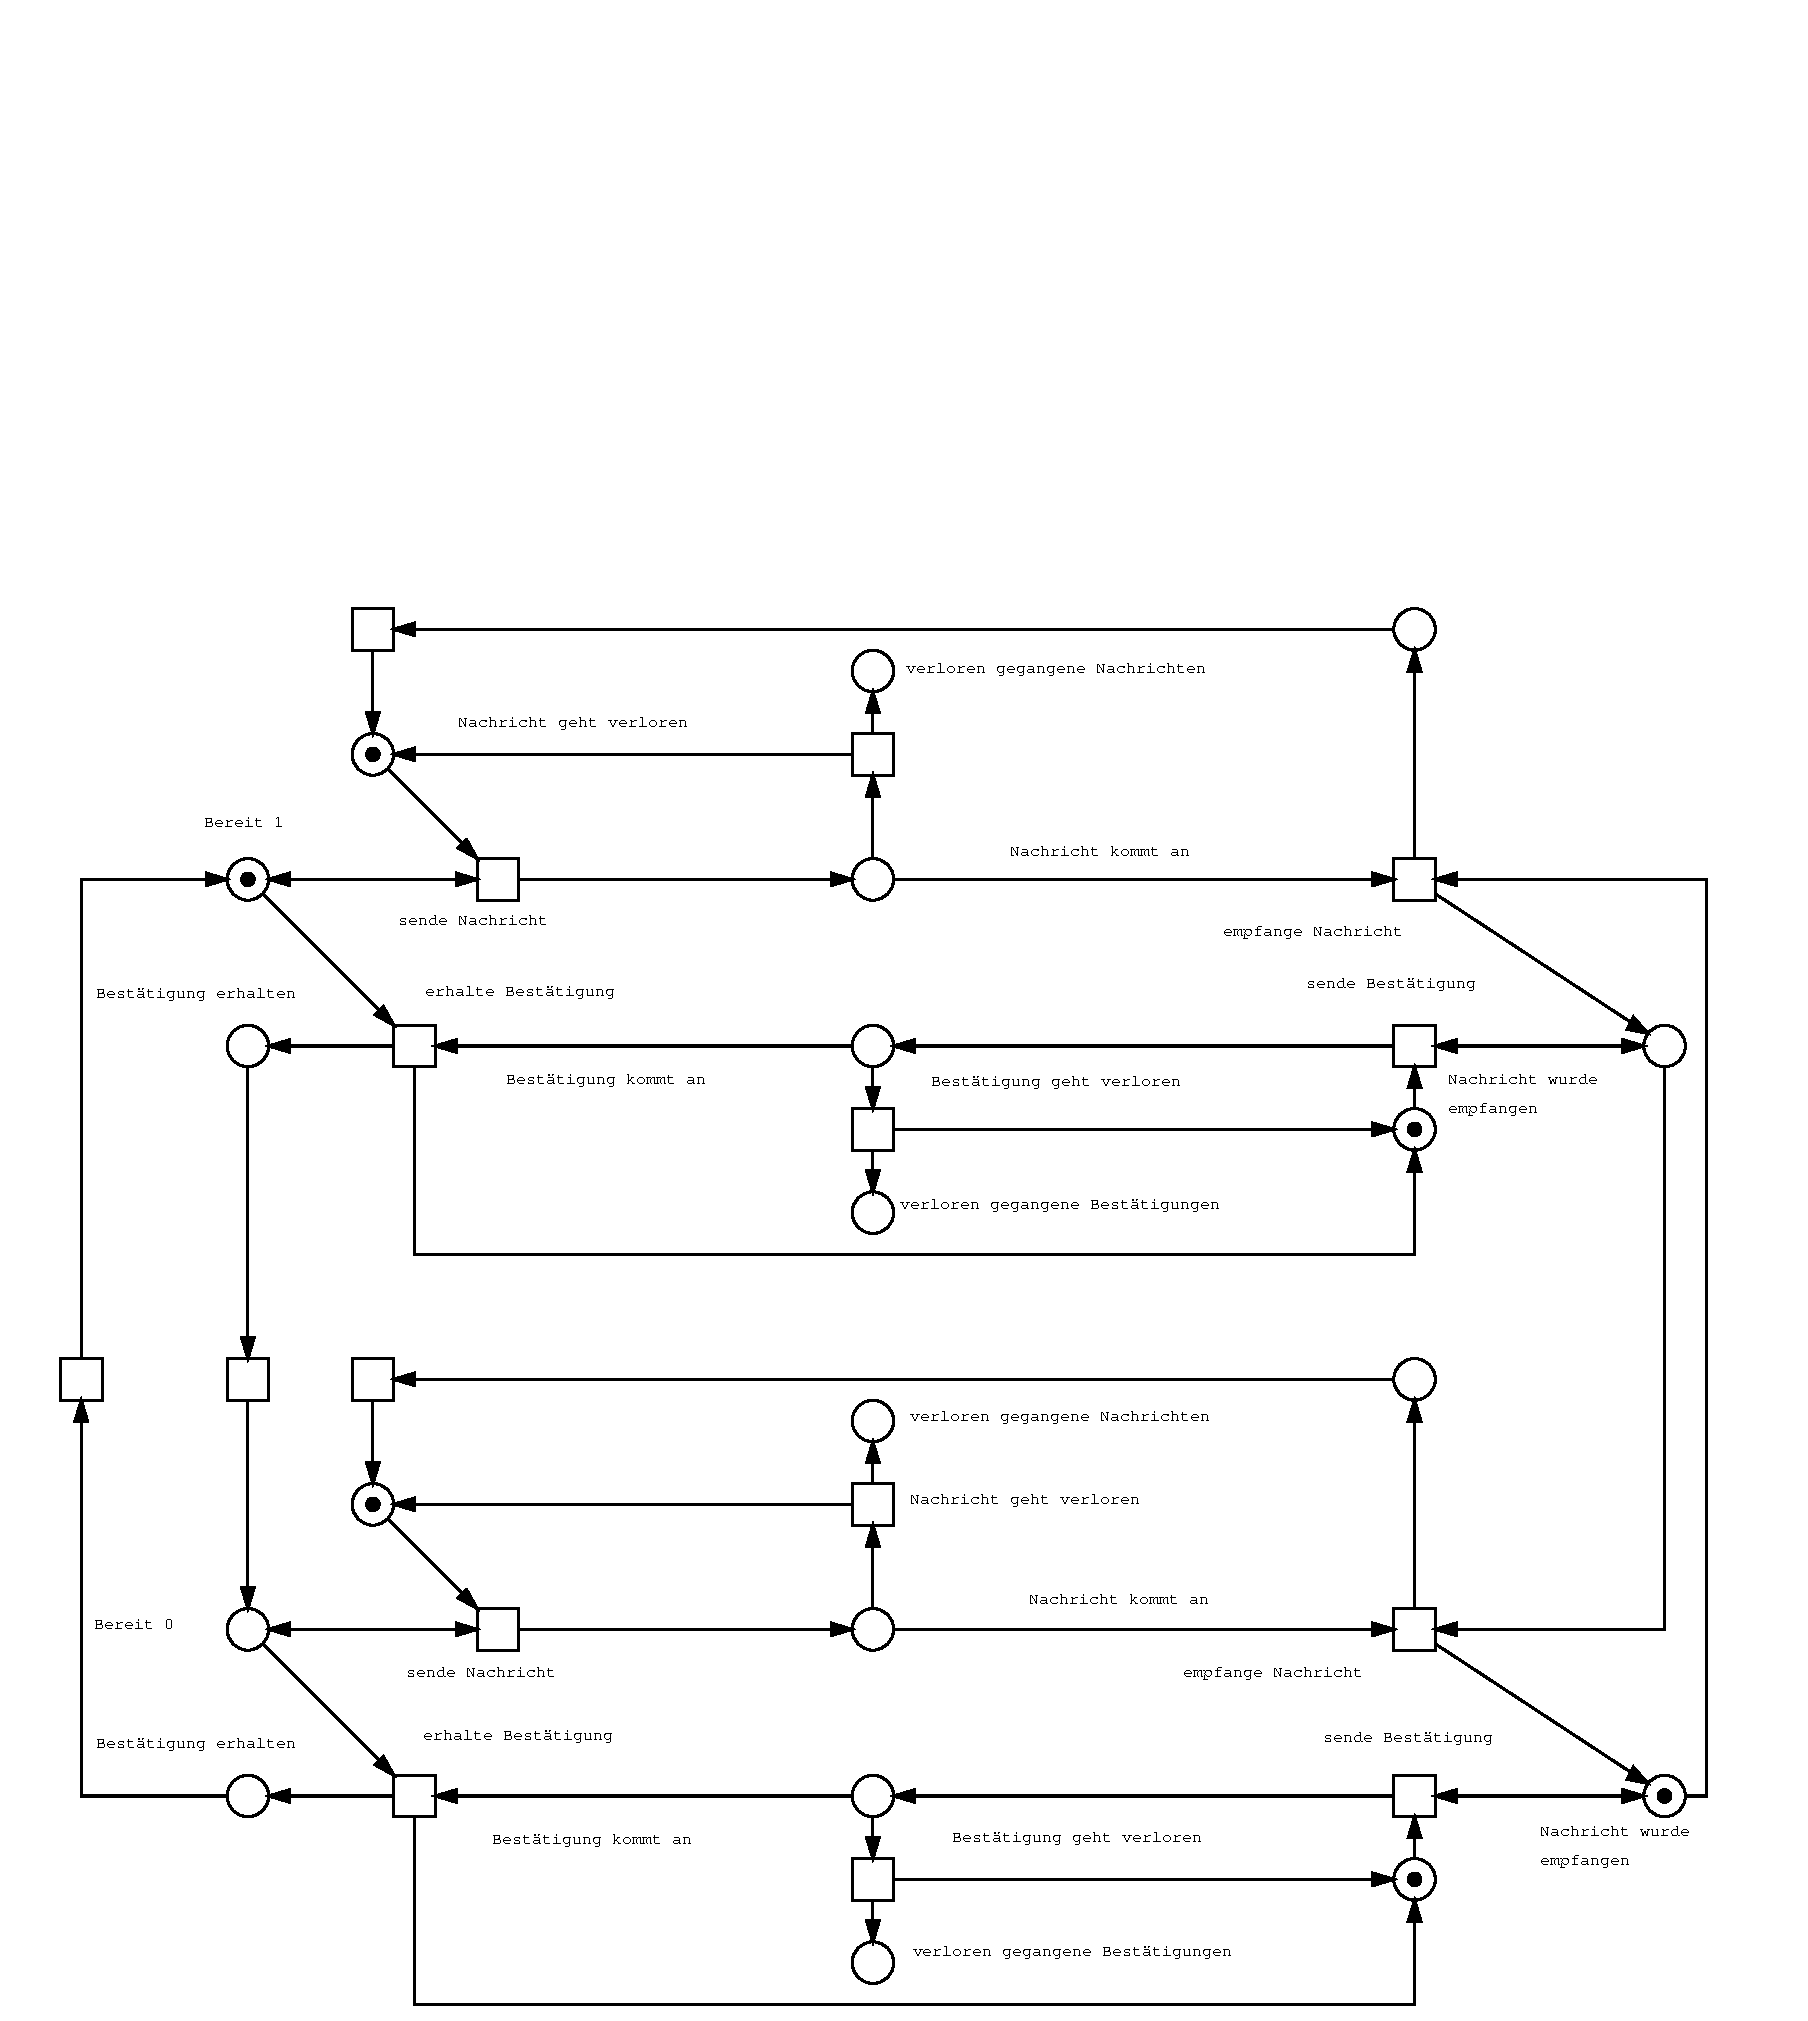
\includegraphics[width=1.0\textwidth]{Bilder/Praktikum1_1.eps}
	\caption{Petrinetz}
	\label{fig:Netz}
\end{figure} 

\subsection{Grundlegender Aufbau}
Abbildung \ref{fig:Netz} zeigt das erstellte Petrinetz zum Alternating Bit Protokoll. Die linke Seite ist die des Senders und die rechte Seite stellt den Empfänger dar. Insgesamt gibt es vier Nachrichtenkanäle die horizontal angeordnet sind. Der oberste Nachrichtenkanal dient dem Versand der Nachricht mit dem Kontrollbit 1 an den Empfänger, wobei im Nachrichtenkanal darunter der Empfang der Nachricht bestätigt wird. Nach Erhalt der Bestätigung wird auf dem dritten Nachrichtenkanal eine Nachricht mit dem Kontrollbit 0 gesendet und ebenfalls bestätigt. Die einzelnen Kanäle haben jeweils eine Stelle in der Mitte der zwei Transitionen zugeordnet sind, dadurch können aufgrund des Nichtdeterminismus Nachrichten verloren gehen. Über Schleifen an den einzelnen Kanälen wird sichergestellt, dass Nachrichten und Bestätigungen solange versendet werden, wie es das Protokoll erfordert.\\

\subsection{Modellierung im Detail}
Die vier wichtigsten Stellen, die das Verhalten des Netzen bestimmen, sind "`Bereit 1"' und "`Bereit 0"' über die das Senden von Nachrichten mit dem jeweiligen Kontrollbit gesteuert wird, sowie die Stellen "`Nachricht wurde empfangen"' auf Empfängerseite über die der Versand der Bestätigungen geregelt wird. Nachfolgend wird kurz auf die einzelnen Stellen und den Ablauf eingegangen.\\
"`Bereit 1"' kennzeichnet die Bereitschaft des Senders, Nachrichten mit dem Kontrollbit 1 zu versenden. Diese Stelle ist zu beginn mit einem Marker besetzt. Nach dem Senden der Nachricht wird der Marker wieder zurück in die Stelle "`Bereit 1"' geschrieben. Als Folge draus ergibt sich, dass der Sender so lange Nachrichten an den Empfänger sendet, bis eine Bestätigung der Nachricht vom Empfänger eintrifft, bei der der Marker aus der Stelle "`Bereit 1"' konsumiert wird.\\
Ähnliches gilt für das Versenden der Bestätigungen an den Sender. Zu Anfang befindet sich in der Stelle "`Nachricht wurde empfangen"' auf Empfängerseite kein Marker, sodass keine Bestätigungen gesendet werden. Erhält der Empfänger nun eine Nachricht vom Sender wird die Stelle "`Nachricht wurde empfangen"' mit einem Marker besetzt und der Empfänger beginnt mit dem Versand von Bestätigungen, solange bis eine Nachricht mit dem invertierten Bit vom Sender eintrifft die den Marker der Stelle "`Nachricht wurde empfangen"' konsumiert.\\
Nachdem die Bestätigung zu der Nachricht mit dem Kontrollbit 1 bei Sender angekommen ist, wird die Stelle "`Bereit 0"' mit einem Marker versehen und der Sender beginnt mit dem Versand von Nachrichten mit dem Kontrollbit 0 bis die Bestätigung zu dieser Nachricht bei ihm eintrifft und der Marker aus "`Bereit 0"' konsumiert wird.\\
Auf Empfängerseite ist die Stelle "`Nachricht wurde empfangen"' zu Beginn besetzt, wodurch der der Empfänger direkt mit dem Versand von Bestätigungen mit dem Kontrollbit 0 beginnt. Die Bestätigungen kommen beim Sender jedoch nicht an, da "`Bereit 0"' nicht mit einem Marker belegt ist. Der Versand "`Geister-Bestätigung"' die ohne Nachrichtenerhalt gestartet wird, endet sobald der Empfänger seine erste Nachricht mit dem Kontrollbit 1 von Sender erhalten hat, da die Transition "`empfange Nachricht"' diesen Marker konsumiert.

\textbf{Aktivierung der Transitionen zu Beginn des Protokolls}

Die Transitionen "`sende Nachricht"' sind M-aktiviert, falls alle Stellen im Vorbereich $\bullet t_{sN}$ einen Marker besitzen.

Die Transition $t_{sN}$ für das Senden der Nachricht mit dem Kontrollbit 1 ist zu Beginn M-aktiviert, da gilt:
\begin{align}
M(\text{Bereit 1}) \geq W(\text{Bereit 1, sende Nachricht}) &\rightarrow 1 \geq 1 & \text{erfüllt} \\
M(\text{Nachricht}) \geq W(\text{Nachricht, sende Nachricht}) &\rightarrow 1 \geq 1 & \text{erfüllt}
\end{align}

Die Transition $t_{sN}$ für das Senden der Nachricht mit dem Kontrollbit 0 ist zu Beginn nicht M-aktiviert, da gilt:
\begin{align}
M(\text{Bereit 0}) \geq W(\text{Bereit 0, sende Nachricht}) &\rightarrow 0 \geq 1 & \text{nicht erfüllt} \\
M(\text{Nachricht}) \geq W(\text{Nachricht, sende Nachricht}) &\rightarrow 1 \geq 1 & \text{erfüllt}
\end{align}

Die Transitionen "`sende Bestätigung"' sind M-aktiviert, falls alle Stellen im Vorbereich $\bullet t_{sB}$ einen Marker besitzen.

Die Transition $t_{sB}$ für das Senden der Bestätigung mit dem Kontrollbit 1 ist zu Beginn nicht M-aktiviert, da gilt:
\begin{align}
M(\text{N. w. empfangen}) \geq W(\text{N. w. empfangen, sende Nachricht}) &\rightarrow 0 \geq 1 & \text{nicht erfüllt} \\
M(\text{Nachricht}) \geq W(\text{Nachricht, sende Nachricht}) &\rightarrow 1 \geq 1 & \text{erfüllt}
\end{align}

Die Transition $t_{sB}$ für das Senden der Bestätigung mit dem Kontrollbit 0 ist zu Beginn M-aktiviert, da gilt:
\begin{align}
M(\text{Nachricht empfangen}) \geq W(\text{Nachricht empfangen, sende Nachricht}) &\rightarrow 1 \geq 1 & \text{erfüllt} \\
M(\text{Nachricht}) \geq W(\text{Nachricht, sende Nachricht}) &\rightarrow 1 \geq 1 & \text{erfüllt}
\end{align}

Somit werden zu Anfang nur Nachrichten mit dem Kontrollbit 1 und Bestätigungen mit dem Kontrollbit 0 versendet, wobei letztere nicht beim Sender ankommen und nur solange gesendet werden, bis die erste Nachricht mit dem Kontrollbit 1 beim Empfänger ankommt und dieser damit dann Bestätigungen mit dem Kontrollbit 1 versendet.

\subsection{Nachrichtenverlust}
Bei einem Versuch sind von 20 gesendeten Nachrichtenpaketen 11 verloren gegangen und 9 angekommen. Diese Verteilung entspricht dem erwarteten Verhalten, da die Stelle die über den Nachrichtenverlust entscheidet zwei Transitionen zu bedienen hat und somit immer nur eine Transition schalten kann. Bei einer fairen Behandlung müssen damit in etwa glich viele Nachrichten ankommen und verloren gehen.

\section{Aufgabe 5 \& 6 - Erweiterung des Systems}
\subsection{Von 20 Nachrichten maximal 1 Nachricht Verlust}
\label{sec:nachrichtenverlust_1}
Um die in der Aufgabe gestellte Anforderung, nicht mehr als eine Nachricht von 20 gesendeten zu verlieren, erfüllen zu können, müssen alle vier Sendeprozesse (Nachrichtenversand mit Bit 1, Nachrichtenversand mit Bit 0, Empfangsbestätigung mit Bit 1 und Empfangsbestätigung mit Bit 0) angepasst werden.\\
Beispielhaft ist in Abbildung \ref{fig:Erweiterung5} die Erweiterung des Prozesses, zum Versand der Nachricht mit Korrekturbit 1, abgebildet.
Ausgehend von der Transition "`empfange Nachricht"' wurde über einer Stelle ein Zähler für die Anzahl empfangener Nachrichten realisiert. 
Die Idee dahinter war es einen Schaltmechanismus zu realisieren, der dafür sorgt, dass sobald eine Nachricht verloren gegangen ist, die nächsten 19 Nachrichten empfangen werden.\\
Zu diesem Zweck wurde die Transition "`Nachricht geht verloren"' um eine weitere Vorbedingung ergänzt, die die Transition nur schalten lässt, wenn nach der ersten verlorenen gegangenen Nachricht 19 Nachrichten erfolgreich empfangen wurden. Die Stelle die dabei als Vorbedingung fungiert besitzt zum Anfang ein Token (eine Nachricht kann damit zu Anfang verloren gehen).
Diese Stelle wurde über eine Transition mit dem Zähler für die empfangenen Nachrichten verbunden.
Die Kante von der Stelle, zum Zählen der empfangenen Nachrichten, hin zur Transition wurde mit einem Gewicht von 19 versehen.
Dieses stellt sicher, dass sobald eine Nachricht verloren gegangen ist, die nächsten 19 empfangen werden.  

\begin{figure}[htbp]
	\centering	\includegraphics[width=1.0\textwidth]{Bilder/Erweiterung_Aufgabe_5}
	\caption{Erweiterung Aufgabe 5}
	\label{fig:Erweiterung5}
\end{figure}

\subsection{Pro gesendeter Nachricht maximal 20 Nachrichten Verlust}
Bei dieser Teilaufgabe wurde ein ähnlicher Ansatz wie in der Vorangegangenen gewählt.
Um die Anforderung realisieren zu können muss die Stelle, die vorher als Schalter agierte, nun die Funktion eins Token Buckets übernehmen.
Das Ziel ist es mit jeder empfangener Nachricht zusätzlich 20 neue Tokens in den Eimer zu tun.
Beim Verlust einer Nachricht wird gleichzeitig ein Token aus dem Eimer konsumiert, so dass Nachrichten nur verloren gehen können wenn der Eimer Tokens enthält.
Das Konstrukt stellt so die Obergrenze von 20 verlorenen Nachrichten sicher.
Der Nichtdeterminismus bestimmt dabei immer noch ob eine Nachricht verloren geht oder empfangen wird.
Diese Mechanismus wird auch bei allen Sendeprozesse realisiert.\\
Im Petrinetz muss hierzu die Lösung aus Abschnitt \ref{sec:nachrichtenverlust_1} mit kleinen Modifikationen versehen werden.
Das Kantengewicht der Vorbedingung der Transition von 19 wird auf 1 gesetzt und die Nachbedingung, also das Kantengewicht der Kante von der Transition zur Stelle die den Eimer darstellt, wird auf 20 gesetzt.
So werden jedes Mal wenn ein Token den Empfänger erreicht 20 neue Tokens in den Token Bucket getan, welches den Verlust von Nachrichten auf 20 pro empfangener Nachricht limitiert. 
 
\begin{figure}[htbp]
	\centering	\includegraphics[width=1.0\textwidth]{Bilder/Erweiterung_Aufgabe_6}
	\caption{Erweiterung Aufgabe 6}
	\label{fig:Erweiterung6}
\end{figure}

\end{document}

